\documentclass{article}
\usepackage{graphicx}
\usepackage{wrapfig}
\usepackage{amsmath}
\usepackage{verbatim}
\usepackage{makeidx}
\usepackage{float}
\usepackage{subfig}
\usepackage[left=1in,top=1in,right=1in]{geometry}

\title{Simulating the Mobot and Linkbot}  
\author{Kevin Gucwa\\Mechanical and Aerospace Engineering}
\date{\today} 
\makeindex

\begin{document}

\begin{center}
{\Huge\sf\bf RoboSim User's Guide}\\
\vspace*{2.5cm}
{\Large\bf Version 0.0.1}
\vspace{4.5cm}
\end{center}

%\maketitle
\newpage
\tableofcontents
\newpage

\section{Introduction}
\texttt{RoboSim} is designed to test programs written to control Barobo Mobot
and Linkbot modules within a simulated environment.  It has been designed to allow
any Ch code which can control hardware Barobo robots to now control them from
within a simulated environment making zero changes the code.  The RoboSim GUI allows
users to change between hardware and simulated robots and position the robots
in their initial position for simulation.

\section{RoboSim GUI}
\label{sec:gui}
The RoboSim gui, shown in Figure \ref{fig:gui}, allows users to configure their computer to run simulated robots
in place of the hardware ones.

\begin{figure}[H]
	\begin{center}
		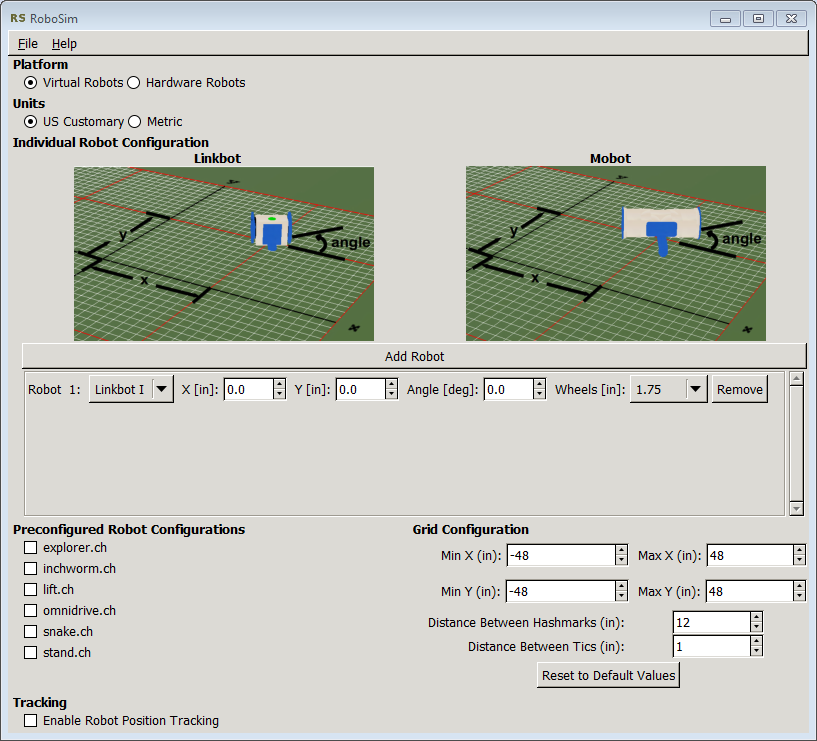
\includegraphics[height=6in]{images/gui}
	\end{center}
	\caption{The RoboSim GUI.}
	\label{fig:gui}
\end{figure}

\subsection{Platform}
This lets a user pick whether the output is sent to the hardware or simulated robots.
\begin{figure}[H]
	\begin{center}
		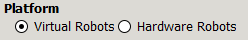
\includegraphics[width=3in]{images/platform}
	\end{center}
	\caption{Initial robot configuration dialog.}
	\label{fig:platform}
\end{figure}

\subsection{Robot Initial Configuration}
To position the robots within the simulation, the user can select a few options which allow
one or two robots to be positioned within the simulated scene.  The options presented provide
the capability of many simple configurations to be tested.  For each of the robots within the scene,
there are five options each of which are outlined below.
\begin{figure}[H]
	\begin{center}
		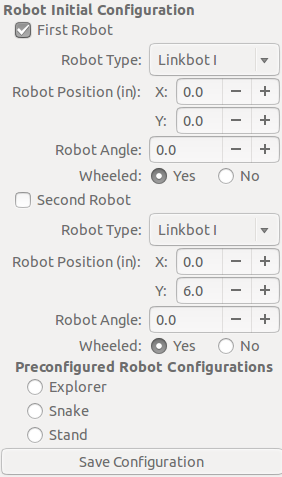
\includegraphics[height=4in]{images/configuration}
	\end{center}
	\caption{Initial robot configuration dialog.}
	\label{fig:config}
\end{figure}

Images for the Mobot and Linkbot showing the meaning of each of the options is
shown to the right of the configuration dialog.

\subsubsection{Robot Type}
There are four options for robot type available.  Linkbot-I, Linkbot-L, Linkbot-T, and Mobot.
The options are presented in a drop down menu as shown in Figure \ref{fig:type}.  Linkbot-T is
a linkbot module with all three joints capable of rotating.

\begin{figure}[H]
	\begin{center}
		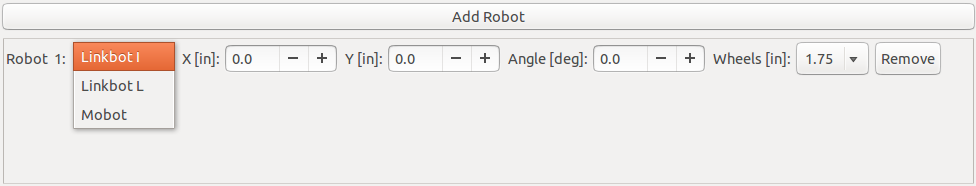
\includegraphics[height=6in]{images/type}
	\end{center}
	\caption{Picking a robot type.}
	\label{fig:type}
\end{figure}

\subsubsection{Robot Position}
Both x and y positions can be chosen independently for each robot.

\subsubsection{Robot Angle}
The rotation angle from the x-axis can be used for changing the orientation of the two robots
respective to each other. 

\subsubsection{Wheels}
Since so many times the robots are run with wheels and a caster connected, a radio button is provided
to build the robots with or without wheels.

\subsubsection{Saving}
The last step is to save the configuration so that Ch can load the information when running any
of the Ch codes.

\section{Running a Simulation}
Once the simulation environment has been configured with the RoboSim GUI in Section \ref{sec:gui}, users
can now run code witten to control the hardware Barobo robots within simulation.  The graphics for
each simulation are created upon running the code.

\section{Interacting with a Simulation}
The simulation window responds to mouse inputs to allow users to move about the scene.
The mouse wheel or right mouse button allows zooming in and out from the robots.  Holding the 
left button rotates the camera about the viewpoint.  Clicking, holding, and dragging both mouse
buttons pans around the scene to change the camera location.

\subsection{Keyboard Input}
The simulation will respond to keyboad input as outlined in Table \ref{tab:keys}.

\begin{table}[H]
	\begin{center}
	\begin{tabular}{c | l }
		\hline \hline
		\textbf{key} & \textbf{action} \\ \hline
		p & Pause and unpause simulation \\
		spacebar & Pause and unpause simulation \\
		\hline \hline
	\end{tabular}
	\caption{Keyboard input for RoboSim}
	\label{tab:keys}
	\end{center}
\end{table}

\appendix
\section{Manual Config File Generation}
\subsection{Robot Attributes}
Each robot element is required to have one attribute titled \textbf{id} which is an unique identifier for the
simulation to reference.  A second optional attribute is \textbf{orientation} which orients the face of a
second robot when it is being attached to a first robot.

\begin{table}[H]
	\begin{center}
	\begin{tabular}{c | l}
		\hline 
		\verb|<linkboti id="0"/>| & one linkbot I with id = 0 \\
		\verb|<linkboti id="0" orientation="3"/>| & Linkbot I is 'upside-down' \\
		\hline
	\end{tabular}
	\caption{Examples}
	\label{tab:ex}
	\end{center}
\end{table}

\begin{table}[H]
	\begin{center}
	\begin{tabular}{c | c | l}
		\hline \hline
		\textbf{attribute} & \textbf{values} & \textbf{description} \\ \hline
		id & unique integer & a unique integer to identify each robot \\
		orientation & 1 & robot face number is at 12 o'clock \\
		 & 2 & robot face number is at 3 o'clock \\
		 & 3 & robot face number is at 6 o'clock \\
		 & 4 & robot face number is at 9 o'clock \\
		\hline \hline
	\end{tabular}
	\caption{Robot Attributes}
	\label{tab:attributes}
	\end{center}
\end{table}

\end{document}
